\chapter{The Search for Invisible Decays of the Higgs Boson}
\label{sec:vbf}

The discovery of the SM Higgs boson~\needcite~involved multiple production modes.
Gluon fusion has the largest cross section (49 pb) at the LHC because of the large gluon PDF, followed by vector boson fusion (VBF) (3.8 pb), $WH$ (1.4 pb), and $ZH$ (0.89 pb)~\cite{lhchxswg}.
While gluon fusion is the most frequent mode, the unique detector signatures of the other production modes can be combined the various Higgs decay signatures to define a signal topology with few backgrounds.

Many DM models~\needcite~allow for DM fermions or scalars to acquire mass through the Higgs mechanism, coupling to the SM Higgs boson.
If the DM candidate $\chi$ satisfies $2m_\chi < m_H$, then we expect to observe $H\rightarrow\chi\bar\chi$.
From measurements of the visible branching fractions, we can indirectly place an upper bound of $\mathcal{B}(H\rightarrow\chi\bar\chi)<0.2$~\needcite.
In this chapter, we describe a direct search for $H\rightarrow\chi\bar\chi$ decays.

As with the case of the mono-top search, the $H\rightarrow\chi\bar\chi$ process manifests as \ptmiss. 
Each of the aforementioned Higgs production modes translates into a $\ptmiss+X$ signature, where $X$ refers to one or more SM particles.
Figure~\ref{fig:vbf:hdiags} shows each of the signatures; in this chapter, we will focus on the VBF production mode, as the unique final state topology provides the best sensitivity to $H\rightarrow\chi\bar\chi$.

\begin{figure}
    \begin{center}
        \begin{subfigure}[t]{0.32\textwidth}
            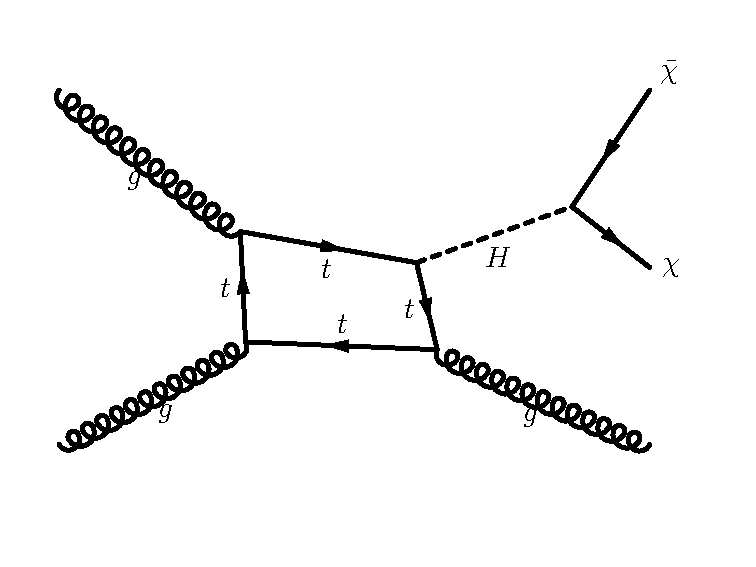
\includegraphics[width=\textwidth]{figures/vbf/diagrams/ggf_hinv.pdf}
            \caption{$gg\rightarrow H(\rightarrow\chi\bar\chi)$+jet(s)}
        \end{subfigure}
        \begin{subfigure}[t]{0.32\textwidth}
            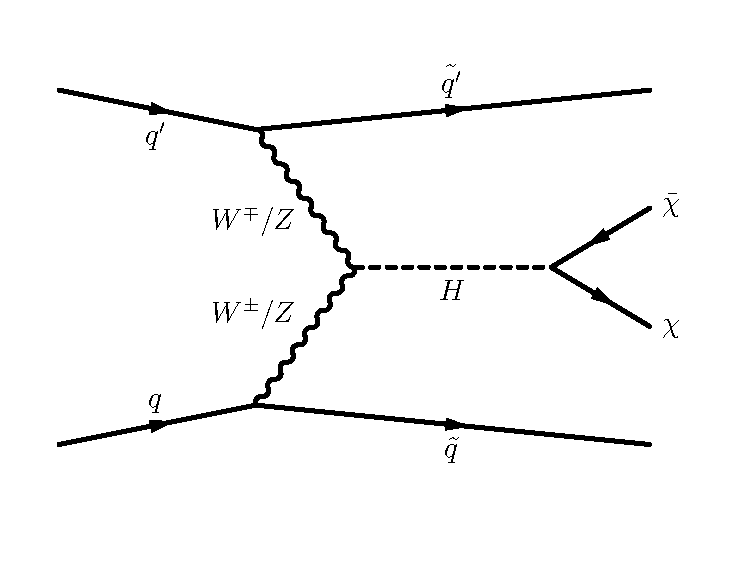
\includegraphics[width=\textwidth]{figures/vbf/diagrams/vbf_hinv.pdf}
            \caption{$qq'\rightarrow H(\rightarrow\chi\bar\chi)$+jet(s)}
        \end{subfigure}
        \begin{subfigure}[t]{0.32\textwidth}
            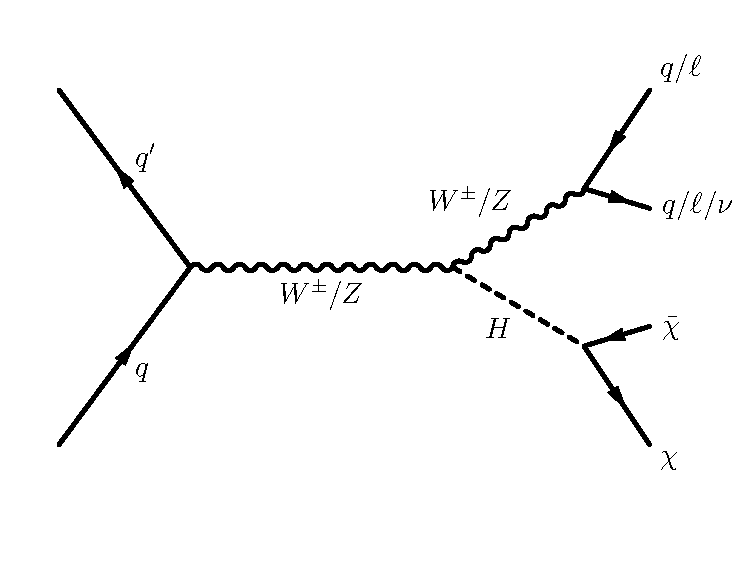
\includegraphics[width=\textwidth]{figures/vbf/diagrams/zh_hinv.pdf}
            \caption{$qq'\rightarrow VH(\rightarrow\chi\bar\chi)$}
        \end{subfigure}
        \caption{Diagrams that contribute to the production of the SM Higgs boson at the LHC, with the subsequent decay to DM candidates.
                 The shown diagrams are all chosen to generate large $\ptmiss$ through the presence of one or more SM particles in the final state.}
        \label{fig:vbf:hdiags}
    \end{center}
\end{figure}

\section{Signal selection}

VBF $\hinv$ events are characterized by large $\ptmiss$ and two jets.
These jets are typically:
\begin{itemize}
    \item Fairly forward in the detector
    \item Far apart from each other in $\eta$
    \item Highly energetic (large $E$, moderate $\pt$)
    \item Close together in $\phi$
\end{itemize}
A candidate VBF $\hinv$ event displaying these properties is shown in a CMS event display in Figure~\ref{fig:vbf:ed}.

\begin{figure}[]
    \begin{center}
        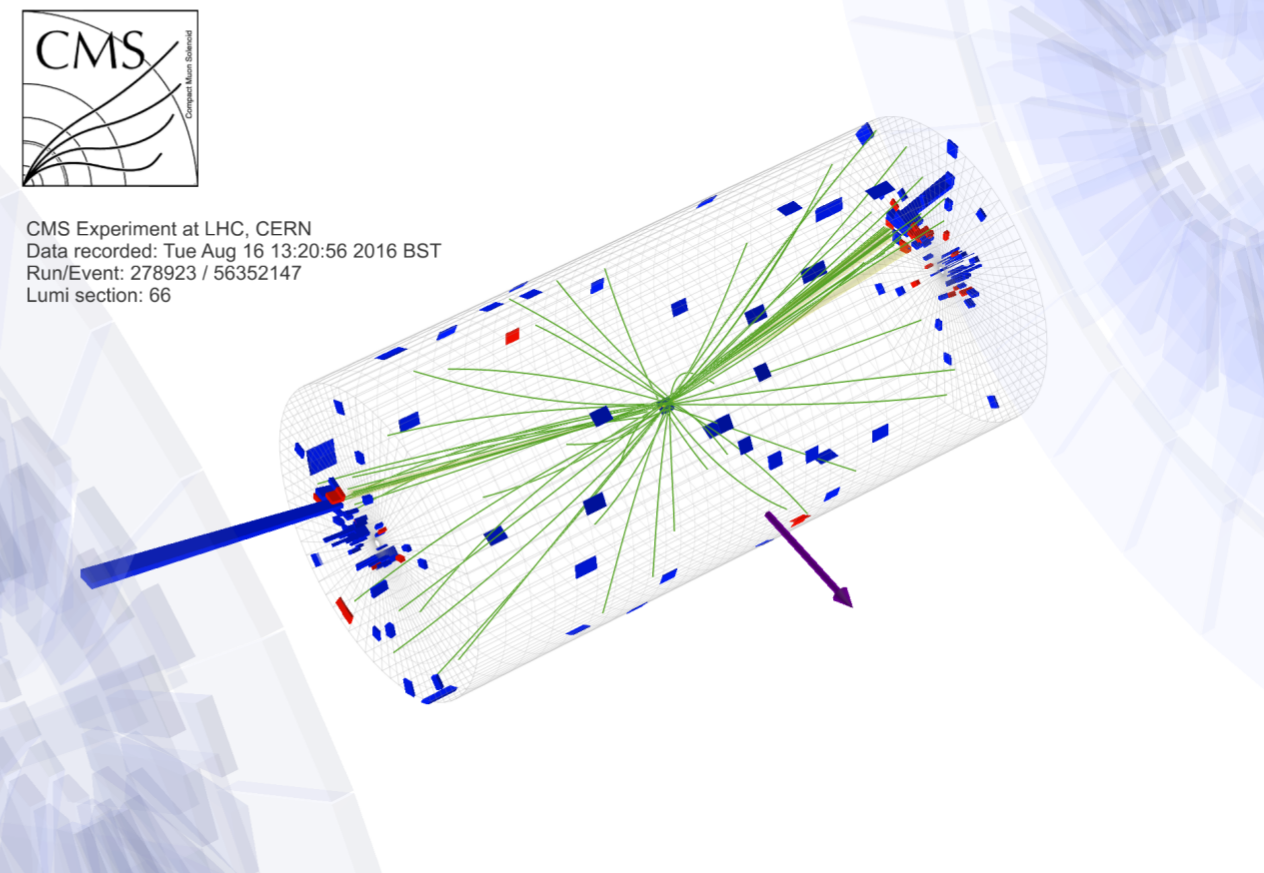
\includegraphics[width=0.8\textwidth]{figures/vbf/misc/event_display.png}
        \caption{Candidate VBF $\hinv$ event with two energetic forward jets ($\pt=180,~107$ GeV) and large $\ptmiss$ ($360$ GeV).
                 Red (blue) towers represent deposits in the hadronic (electromagnetic) calorimeter.
                 Green lines are tracks reconstructed from hits of charged particles in the tracker. 
                 The blue arrow represents the direction and magnitude of the $\ptmiss$.}
        \label{fig:vbf:ed}
    \end{center}
\end{figure}

\subsection{Online trigger selection}

The same trigger decisions (L1 and HLT) as described in Section~\ref{sec:mt:trigger} are used to select events in this analysis.
However, the L1 seeds for the 2016 data run were designed with mono-top-like analyses in mind; i.e., searches where the momentum imbalance is created by central objects.
To avoid noise and resolution issues in the forward calorimeters, the L1 seed only considers energy deposits in the region ${|\eta|<3}$. 
Therefore, VBF events in which both jets are in the forward region are not selected.  

This is visible in Figure~\ref{fig:vbf:hlta}, where events are classified based on the location of the two highest-$\pt$ jets.
Events with both jets in the barrel (BB) have a higher efficiency than events with one jet in the forward detector (BF).
Note that events with two forward jets (FF) are not considered at all, as the efficiency for such events is essentially zero. 

\begin{figure}[]
    \begin{center}
        \begin{subfigure}[t]{0.49\textwidth}
            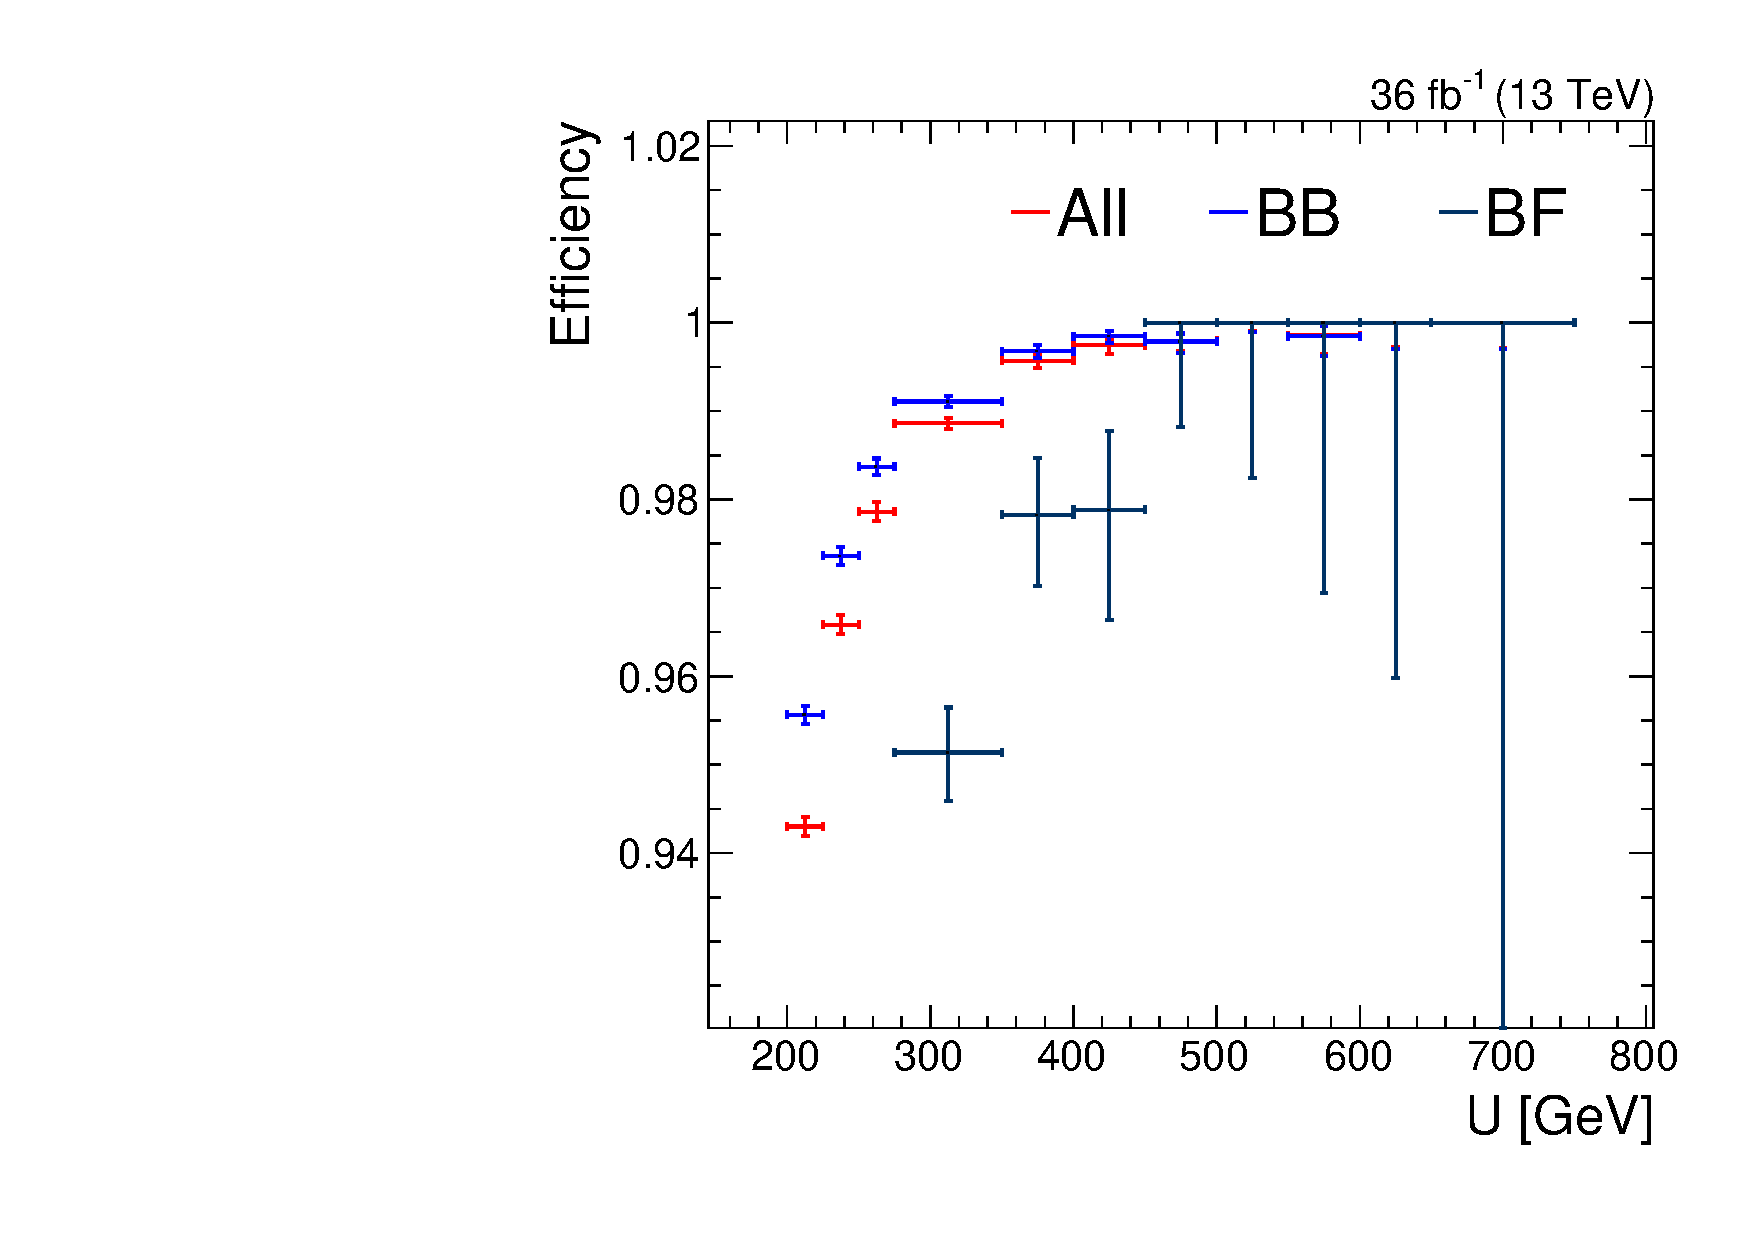
\includegraphics[width=\textwidth]{figures/vbf/triggers/trigeff_nmu1pfUWmag.pdf}
            \caption{Recoil}
            \label{fig:vbf:hlta}
        \end{subfigure}
        \begin{subfigure}[t]{0.49\textwidth}
            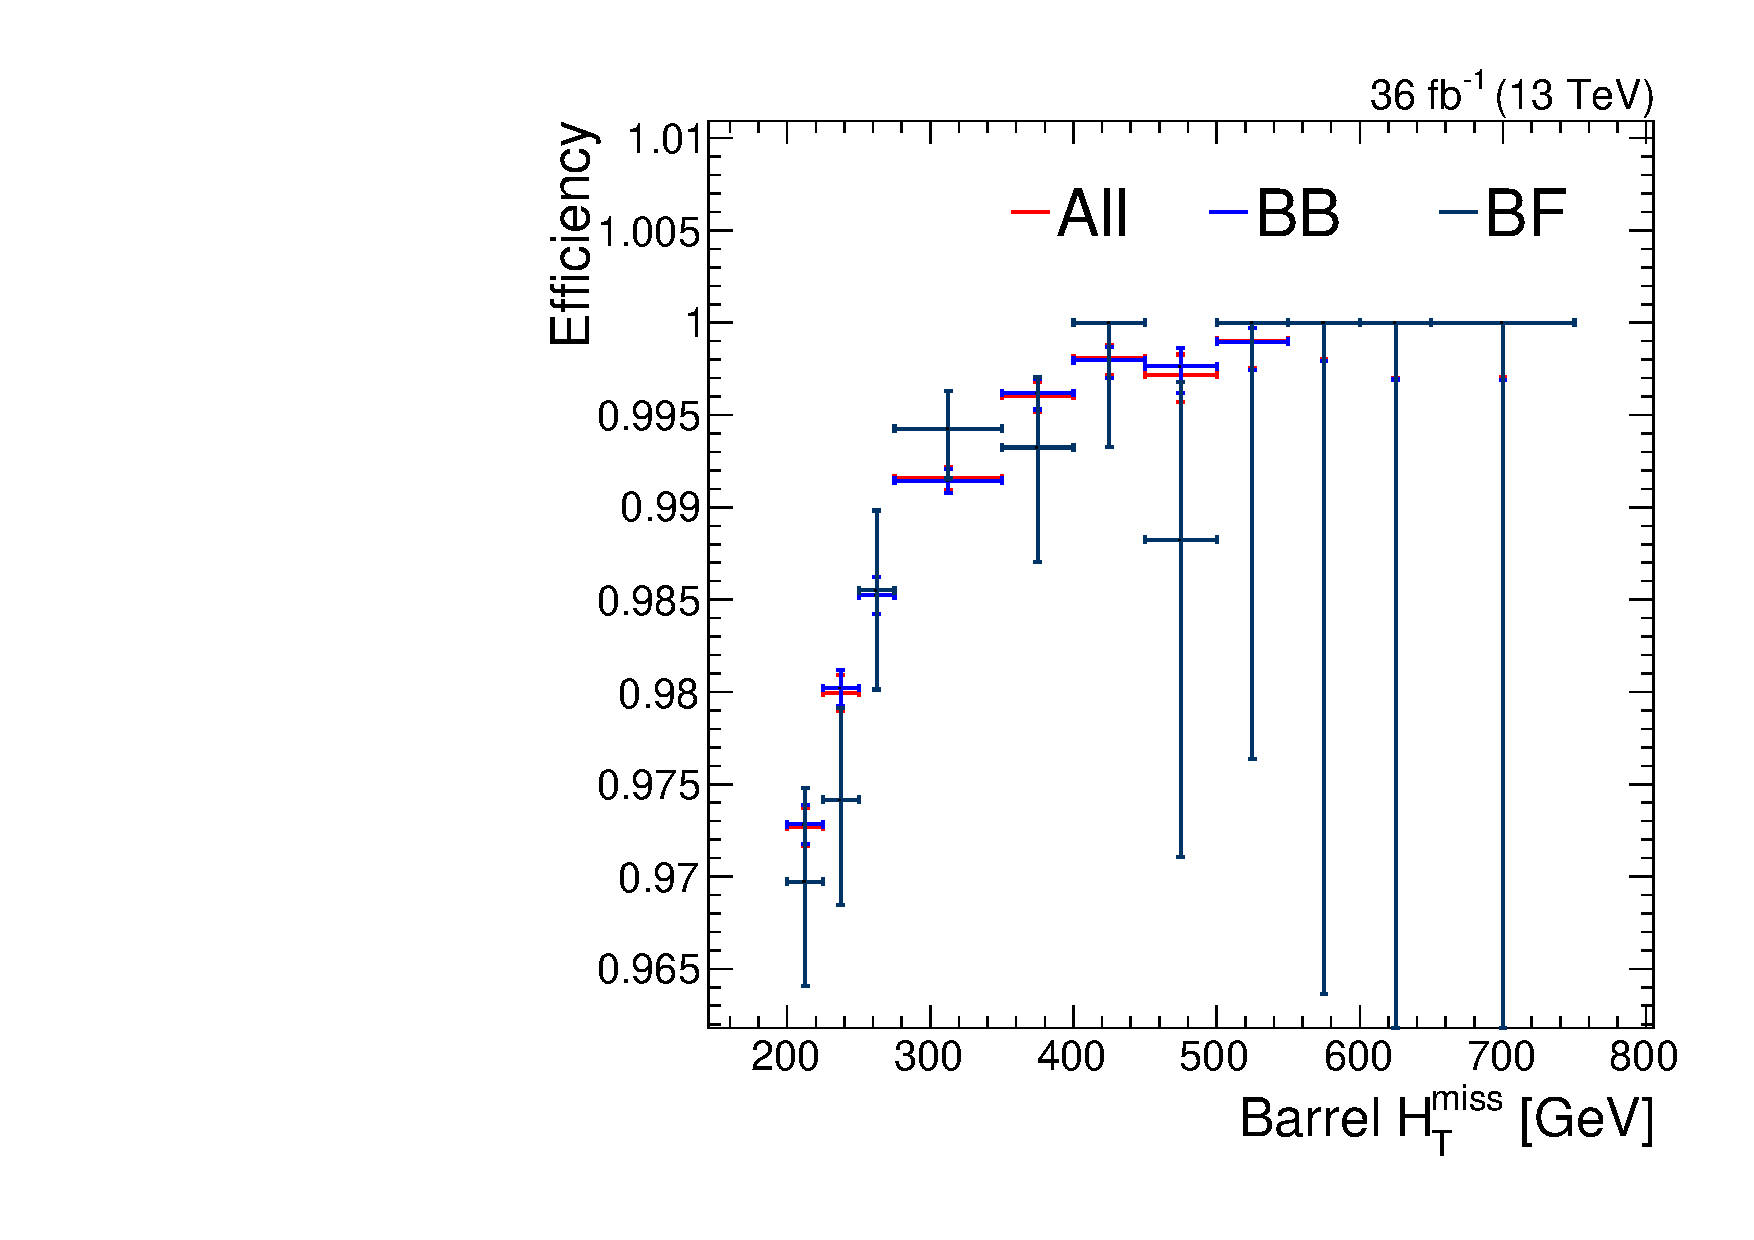
\includegraphics[width=\textwidth]{figures/vbf/triggers/trigeff_nmu1barrelHTMiss.pdf}
            \caption{$H_\mathrm{T,barrel}^\mathrm{miss}$}
            \label{fig:vbf:hltb}
        \end{subfigure}
        \caption{Trigger efficiency of events with a VBF-like topology (two jets with $\pt>80,40$ GeV) as a function of two different observables.
                 Events are split into two categories: those where both jets have $|\eta|<3$ (BB) and those were exactly one jet has $|\eta|>3$ (FF).
                 "All" refers to the sum of these categories.}
        \label{fig:vbf:hlt}
    \end{center}
\end{figure}

The trigger efficiency is truly characterized by the energy deposited in the $|\eta|<3$ region of the detector, and will be dominated in VBF events by the energy of jets.
Accordingly, we define the ``missing barrel hadronic transverse momentum'':
\begin{equation}
    H_\mathrm{T,barrel}^\mathrm{miss} = \left|\left(\sum_{j\in\text{barrel}} \vec{p}_j \right)_\mathrm{T}\right|, \text{ where barrel refers to jets with $|\eta|<3$}
\end{equation}
As shown in Figure~\ref{fig:vbf:hltb}, the three categories (BB, BF, All) have similar behavior as a function of $H_\mathrm{T,barrel}^\mathrm{miss}$.
Therefore, we use this parameterization of the efficiency to correct MC simulation to match data. 

A second L1-related issue that plagues the 2016 dataset is caused by a ``pre-firing'' effect.
When an L1 seed is triggered to accept an event (``L1Accept'' or ``L1A''), the following two bunch crossings (not necessarily corresponding to collisions) are blocked from firing L1As. 
At most, two in four consecutive events can fire L1A (i.e. the sequence L1A, blocked, blocked, L1A).
Figure~\ref{fig:vbf:pre1} is an example of a normal ECAL L1 seed accepting an event and blocking the subsequent bunch crossings.
In what follows, we will refer to the bunch crossing with an interesting collision (i.e. the one we would like the trigger to select) as \bx{0}.

\begin{figure}
    \begin{center}
        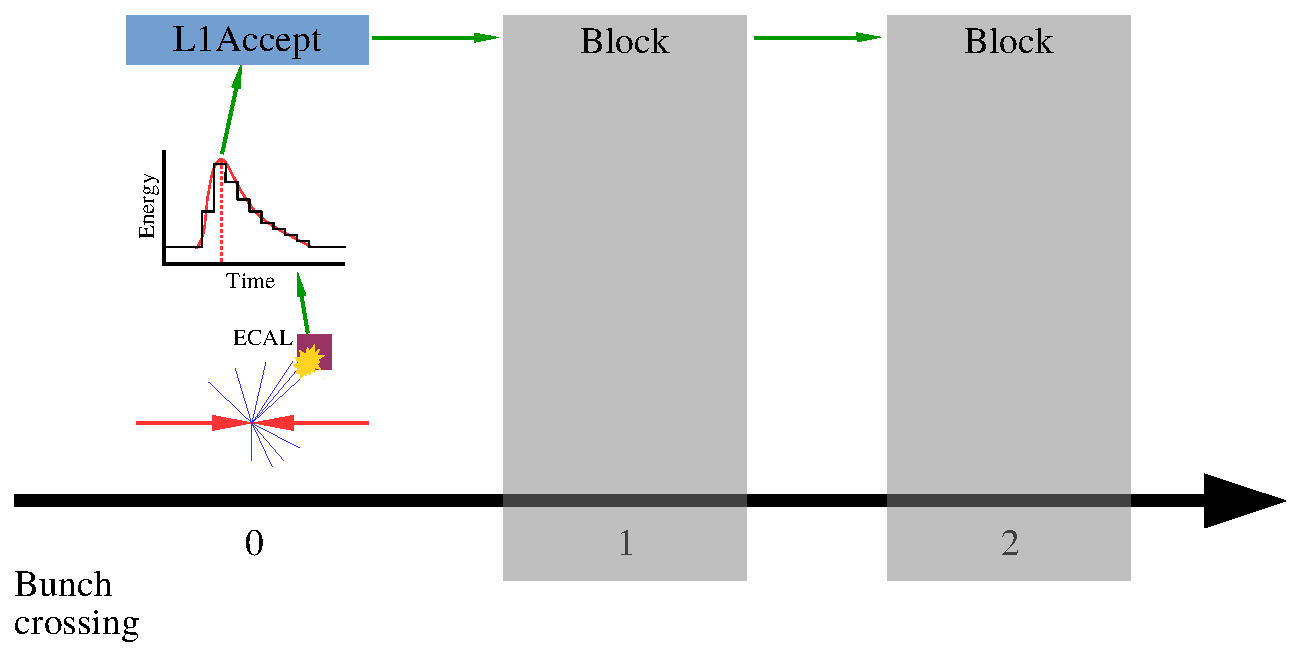
\includegraphics[width=0.8\textwidth,page=1]{figures/vbf/triggers/l1diag.pdf}
        \caption{A normal event in which an ECAL seed triggers the L1A signal. 
                 The subsequent two bunch crossings are blocked. 
                 \bx{0}~refers to the event containing the physics object of interest.
                 Green arrows indicate causality.}
        \label{fig:vbf:pre1}
    \end{center}
\end{figure}

A pre-fire refers to the case in which a malformed detector signal is mis-reconstructed, so that the peak of the pulse appears to have occurred in the previous bunch crossing (\bx{-1}).   
In this particular case, a region of the ECAL ($2.5 < |\eta|<3$) suffered from a loss in transparency due to radiation damage and would produce pulse shapes that are poorly described by the model used to extract the pulse energy and time. 
When this happens, the L1 seeds for ECAL-based signatures (e.g. electron triggers) can fire an L1A for \bx{-1}.
So, we would have an L1A for an arbitrary event (\bx{-1}), and the interesting event (\bx{0}) would be blocked from passing the L1 altogether. 
This is depicted in Figure~\ref{fig:vbf:pre2}.
Typically, \bx{-1}~contains uninteresting physics signatures, and so is not accepted by the HLT.

\begin{figure}
    \begin{center}
        \includegraphics[width=0.8\textwidth,page=2]{figures/vbf/triggers/l1diag.pdf}
        \caption{A pre-fired event in which an ECAL seed triggers the L1A signal for \bx{-1}. 
                 The subsequent two bunch crossings (including the one of interest) are blocked. 
                 \bx{0}~refers to the event containing the physics object of interest.
                 Green arrows indicate causality.}
        \label{fig:vbf:pre2}
    \end{center}
\end{figure}

To measure how often an ECAL energy deposit (typically left by a jet) causes an event to be lost by pre-firing, we need to compute the following efficiency:
\begin{equation}
    \epsilon_\text{pre-fire}(\pt,\eta,\phi) = \frac{N_\text{pre-fire}(\pt,\eta,\phi)}{N_\text{all events}(\pt,\eta,\phi)}
\end{equation}
However, by definition, pre-fired events cannot be recorded, and therefore $N_\text{pre-fire}(\pt,\eta,\phi)$ is difficult to measure.
A very small subset of the recorded dataset ($0.2\%$) consists of ``un-pre-fireable'' events.
These are recorded events (\bx{0}) in which an L1A fired 3 bunch crossings prior (\bx{-3}).
Due to the blocking rules, L1A cannot fire in \bx{-2}~and \bx{-1}.
Even if there is an ECAL seed in \bx{0}~that pre-fires, it will be blocked from firing an L1A, and therefore \bx{0}~is protected.
If some other object in \bx{0}~manages to pass L1 and HLT decisions, then \bx{0}~will be recorded and can be studied.
A schematic of such events is shown in Figure~\ref{fig:vbf:pre3}.

\begin{figure}
    \begin{center}
        \includegraphics[width=0.8\textwidth,page=3]{figures/vbf/triggers/l1diag.pdf}
        \caption{An un-pre-fireable event in which \bx{-3}~protects \bx{0}~from being pre-fired. 
                 Green arrows indicate causality.}
        \label{fig:vbf:pre3}
    \end{center}
\end{figure}

The L1 trigger system records trigger primitive (TP) information (4-vectors of physics objects considered in an L1 selection) for \bx{-1}~if \bx{0}~is triggered.
This means we can identify the cases in which a physics object in \bx{0}~coincides with a TP in \bx{-1}, indicating a pre-fire. 
Therefore (using the bunch crossing numbering in Figure~\ref{fig:vbf:pre3}), we re-define the efficiency:
\begin{equation}
    \epsilon_\text{pre-fire}(\pt,\eta,\phi) = \frac{N_\text{pre-fire \bx{0}|\bx{-3}}(\pt,\eta,\phi)}{N_\text{\bx{0}|\bx{-3}}(\pt,\eta,\phi)}
\end{equation}
By definition, all events in this ratio will be recorded. 
Figure~\ref{fig:vbf:pre_eff2_etaphi} shows this efficiency as a function of jet location. 
We observe there is a ``hot'' ECAL tower near the location $\eta=-2.8$ and $\phi=2$.
Not only does this tower fire very frequently (leading to many particles, leading to many jets), but it almost always pre-fires.
To first order, events with a jet in this crystal should be rejected.
Beyond this, there is very little localization in the pre-fire probability (besides restriction to the ECAL endcap). 

\begin{figure}[]
    \begin{center}
        \begin{subfigure}[t]{0.49\textwidth}
            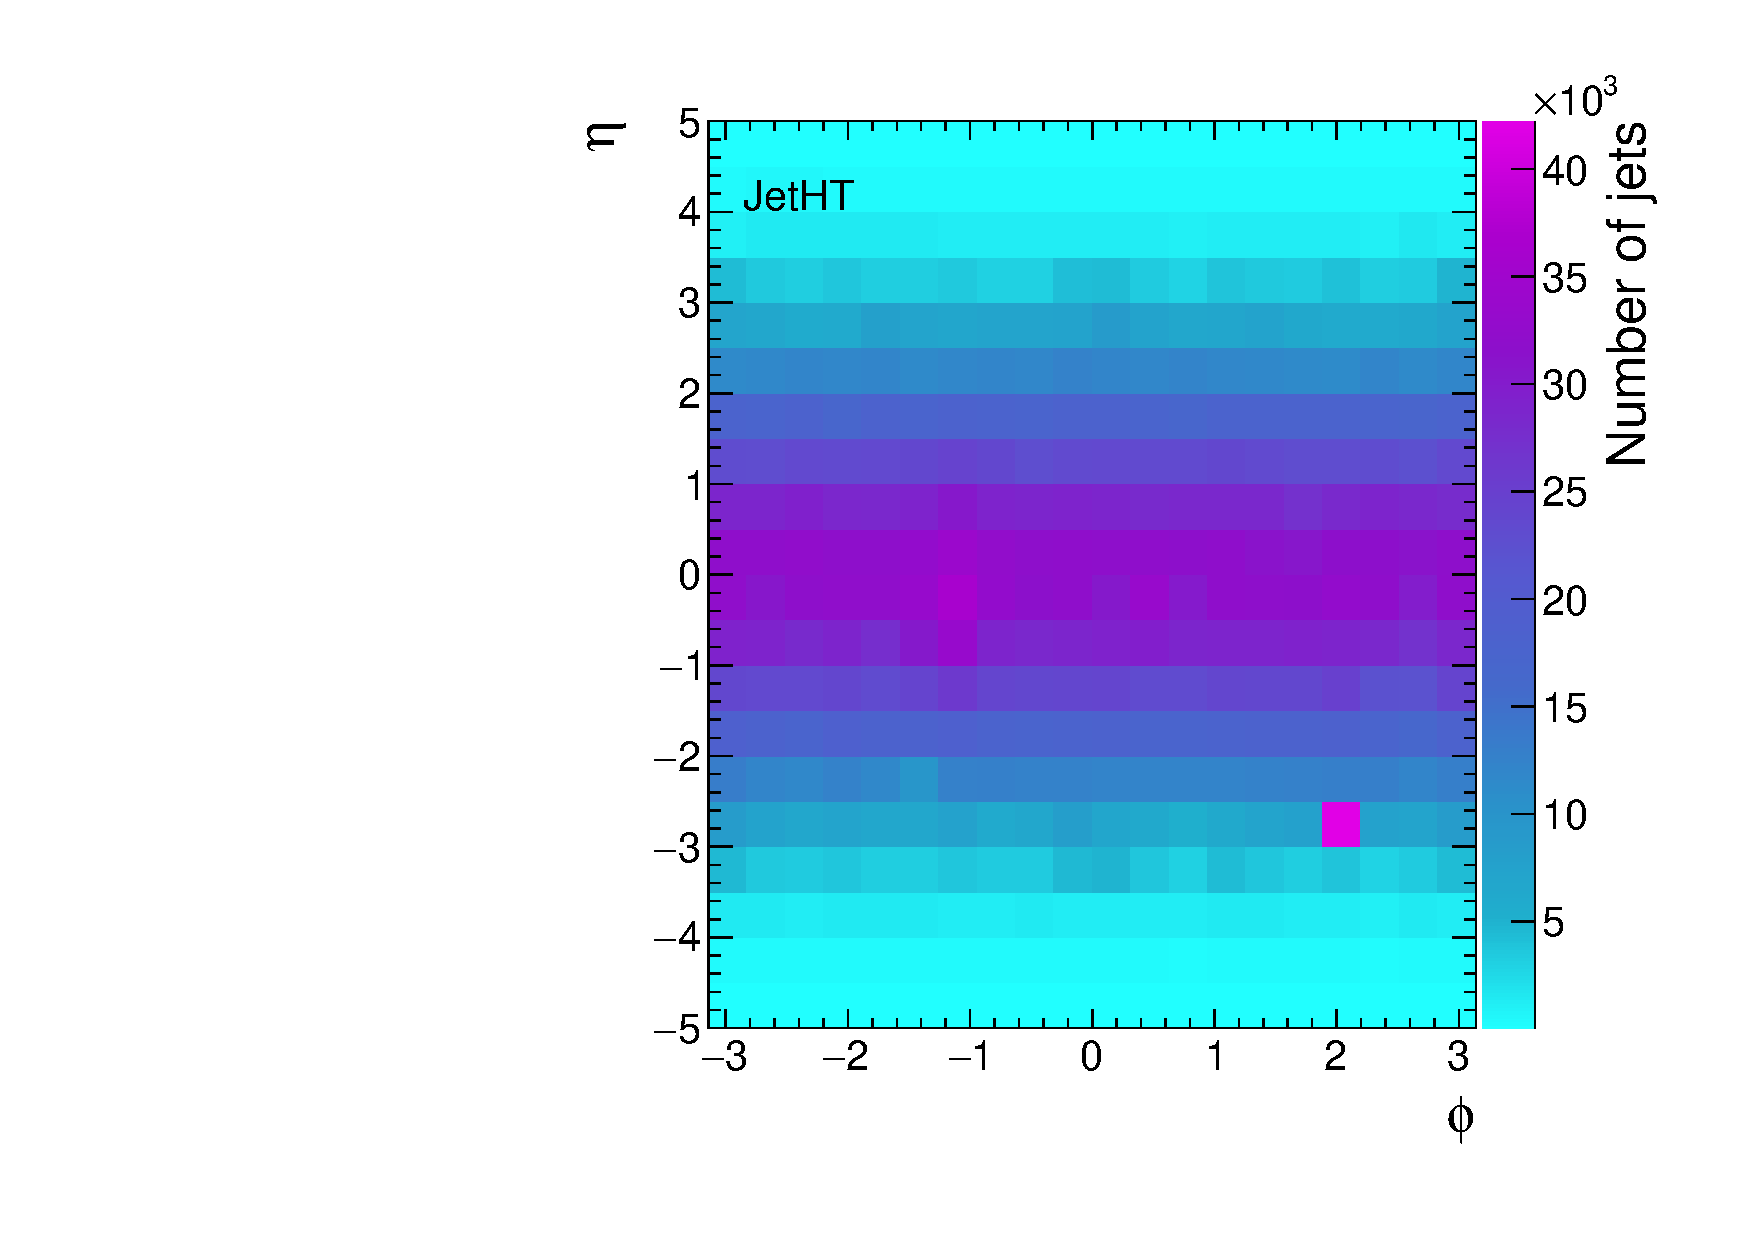
\includegraphics[width=\textwidth]{figures/vbf/triggers/JetHT_inclusive_egiso_etaphi_den.pdf}
            \caption{Number of jets}
            \label{fig:vbf:hlta}
        \end{subfigure}
        \begin{subfigure}[t]{0.49\textwidth}
            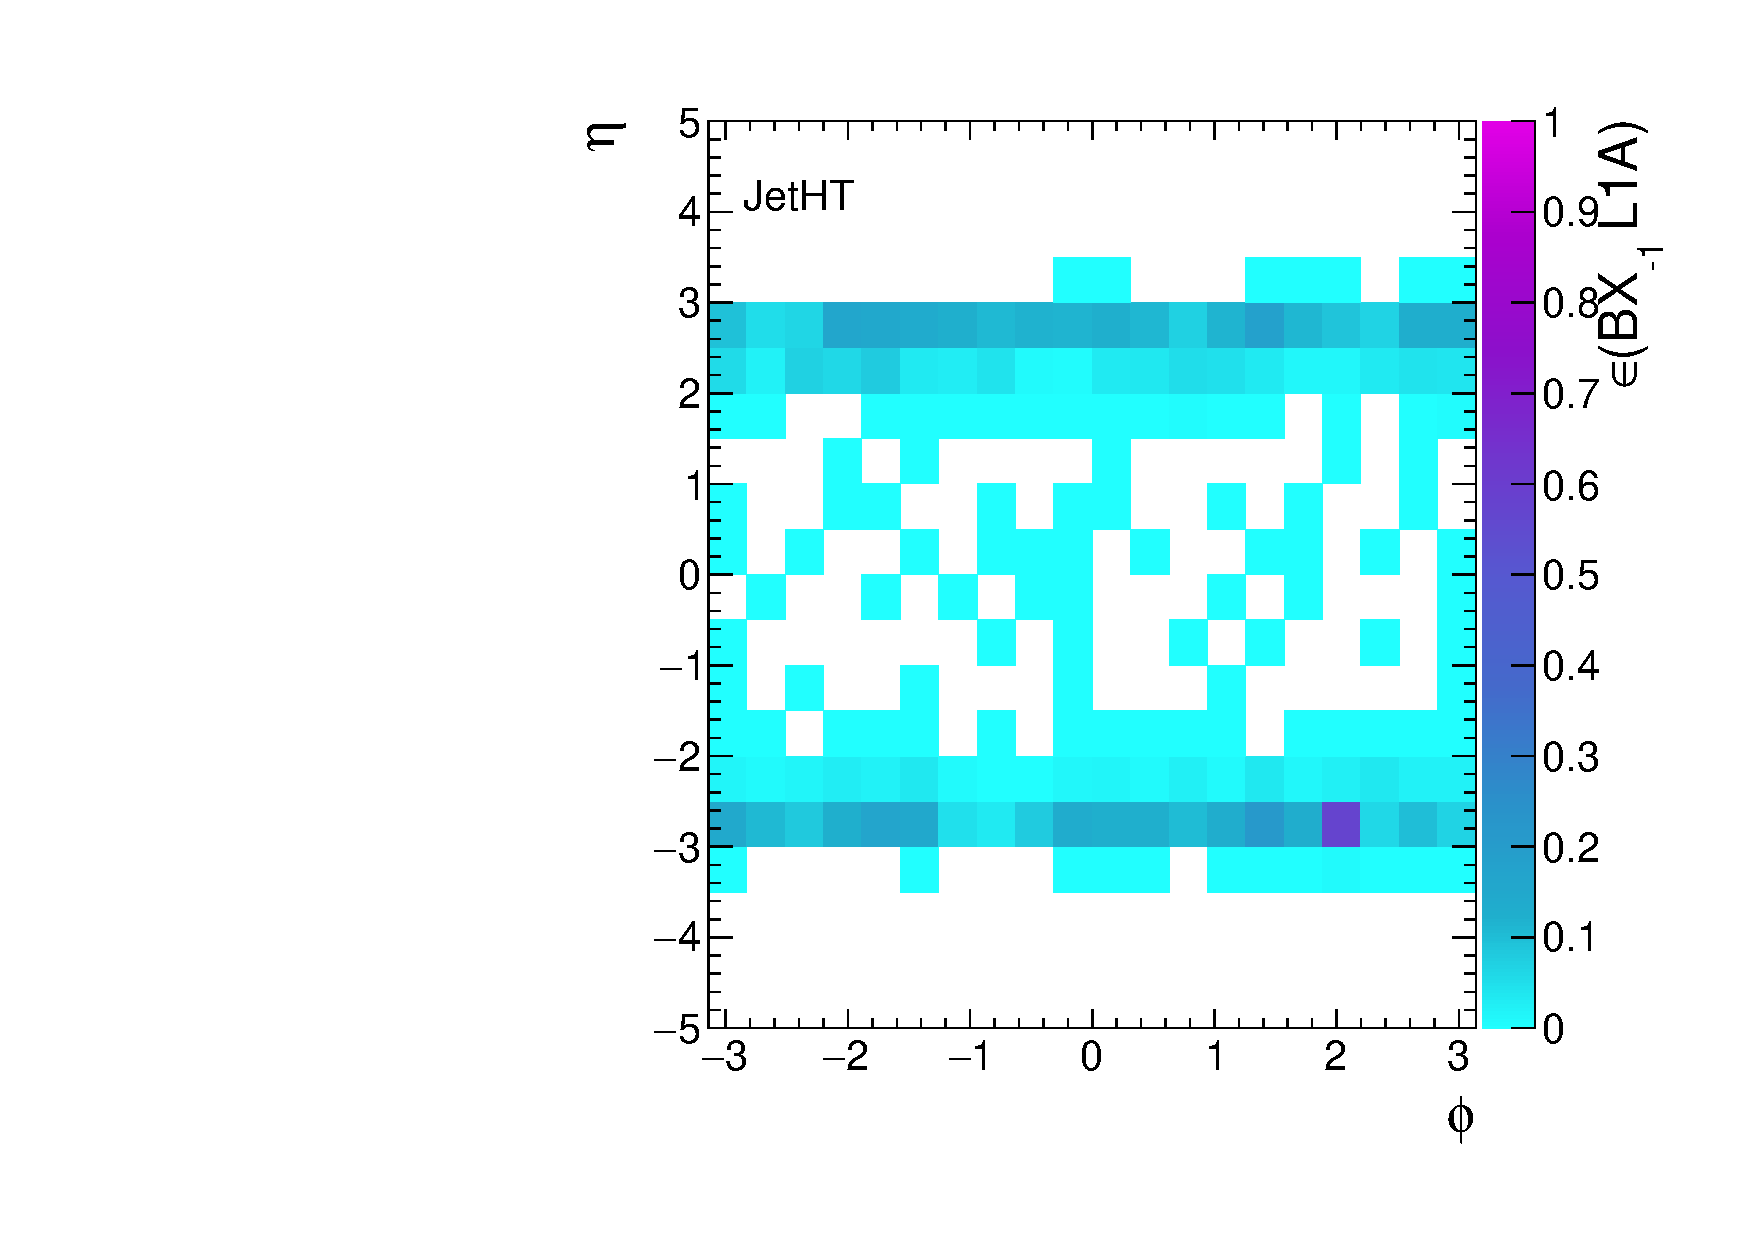
\includegraphics[width=\textwidth]{figures/vbf/triggers/JetHT_inclusive_egiso_etaphi_ratio.pdf}
            \caption{Pre-fire probability}
            \label{fig:vbf:hltb}
        \end{subfigure}
        \caption{Distribution of jets and pre-fire events as a function of the jet location in the detector.
                 Note the spike near $(\eta,\phi) = (-2.8,2)$. }
        \label{fig:vbf:pre_eff2_etaphi}
    \end{center}
\end{figure}

In Figure~\ref{fig:vbf:pre_eff1} we see $\epsilon_\text{pre-fire}$ as a function of $\pt$ in a restricted $\eta$ range.
Firstly, we observe that $\epsilon_\text{pre-fire}$ increases as a function of $\pt$, and the turn-on is sharper as a function of EM $\pt$. 
This is explained by the mechanism of the pre-fire: the individual ECAL trigger seeds have a threshold of 30 GeV.
The higher the jet $\pt$, the higher the probability of the jet depositing $30$ GeV of EM energy in a localized area, setting off an L1 seed. 
Secondly, we observe a strong dependence on the reference triggers used to select $\bx{0}$.
For example, jet-based triggers (JetHT) lead to a much higher efficiency than $\ptmiss$-based triggers (MET).  

\begin{figure}[]
    \begin{center}
        \begin{subfigure}[t]{0.49\textwidth}
            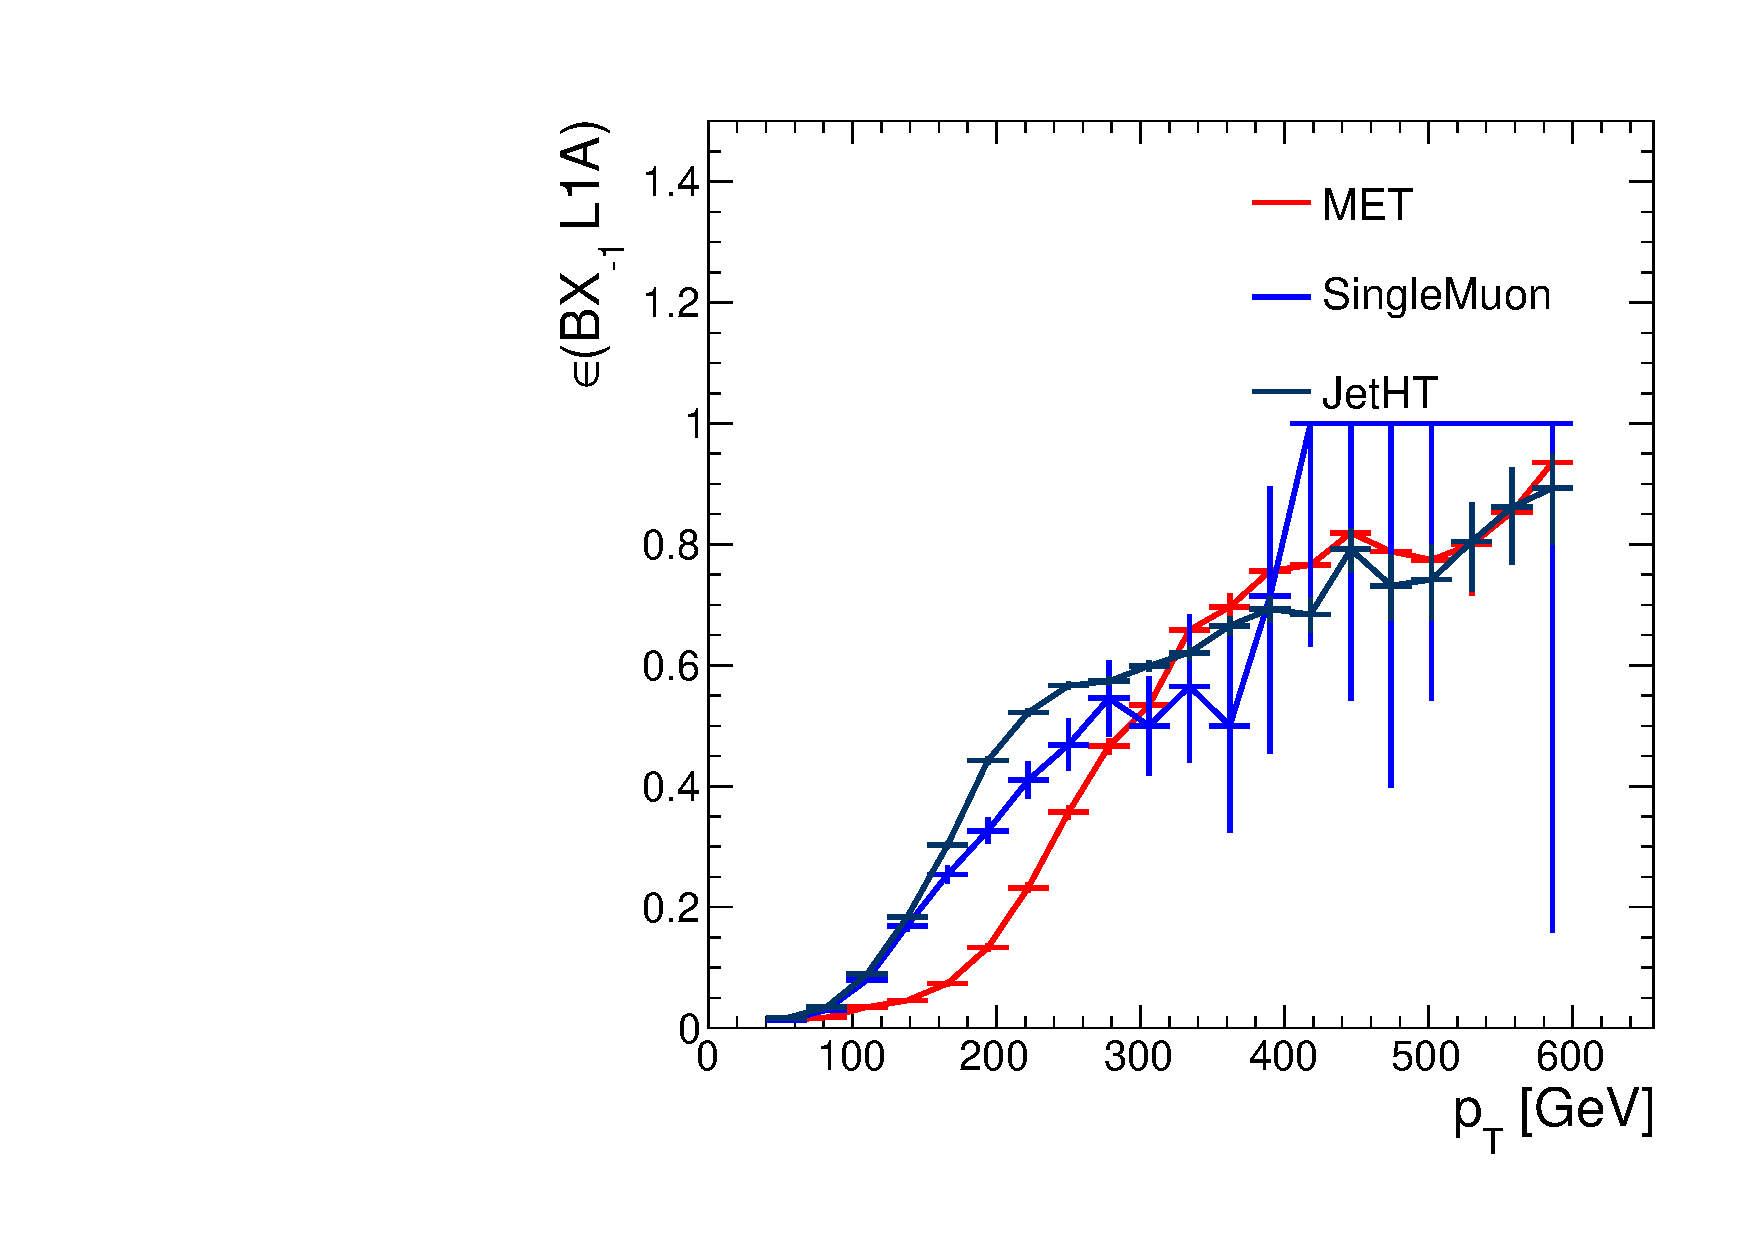
\includegraphics[width=\textwidth]{figures/vbf/triggers/oned_jotPt_finor_ratio.pdf}
            \caption{$\pt$}
            \label{fig:vbf:hlta}
        \end{subfigure}
        \begin{subfigure}[t]{0.49\textwidth}
            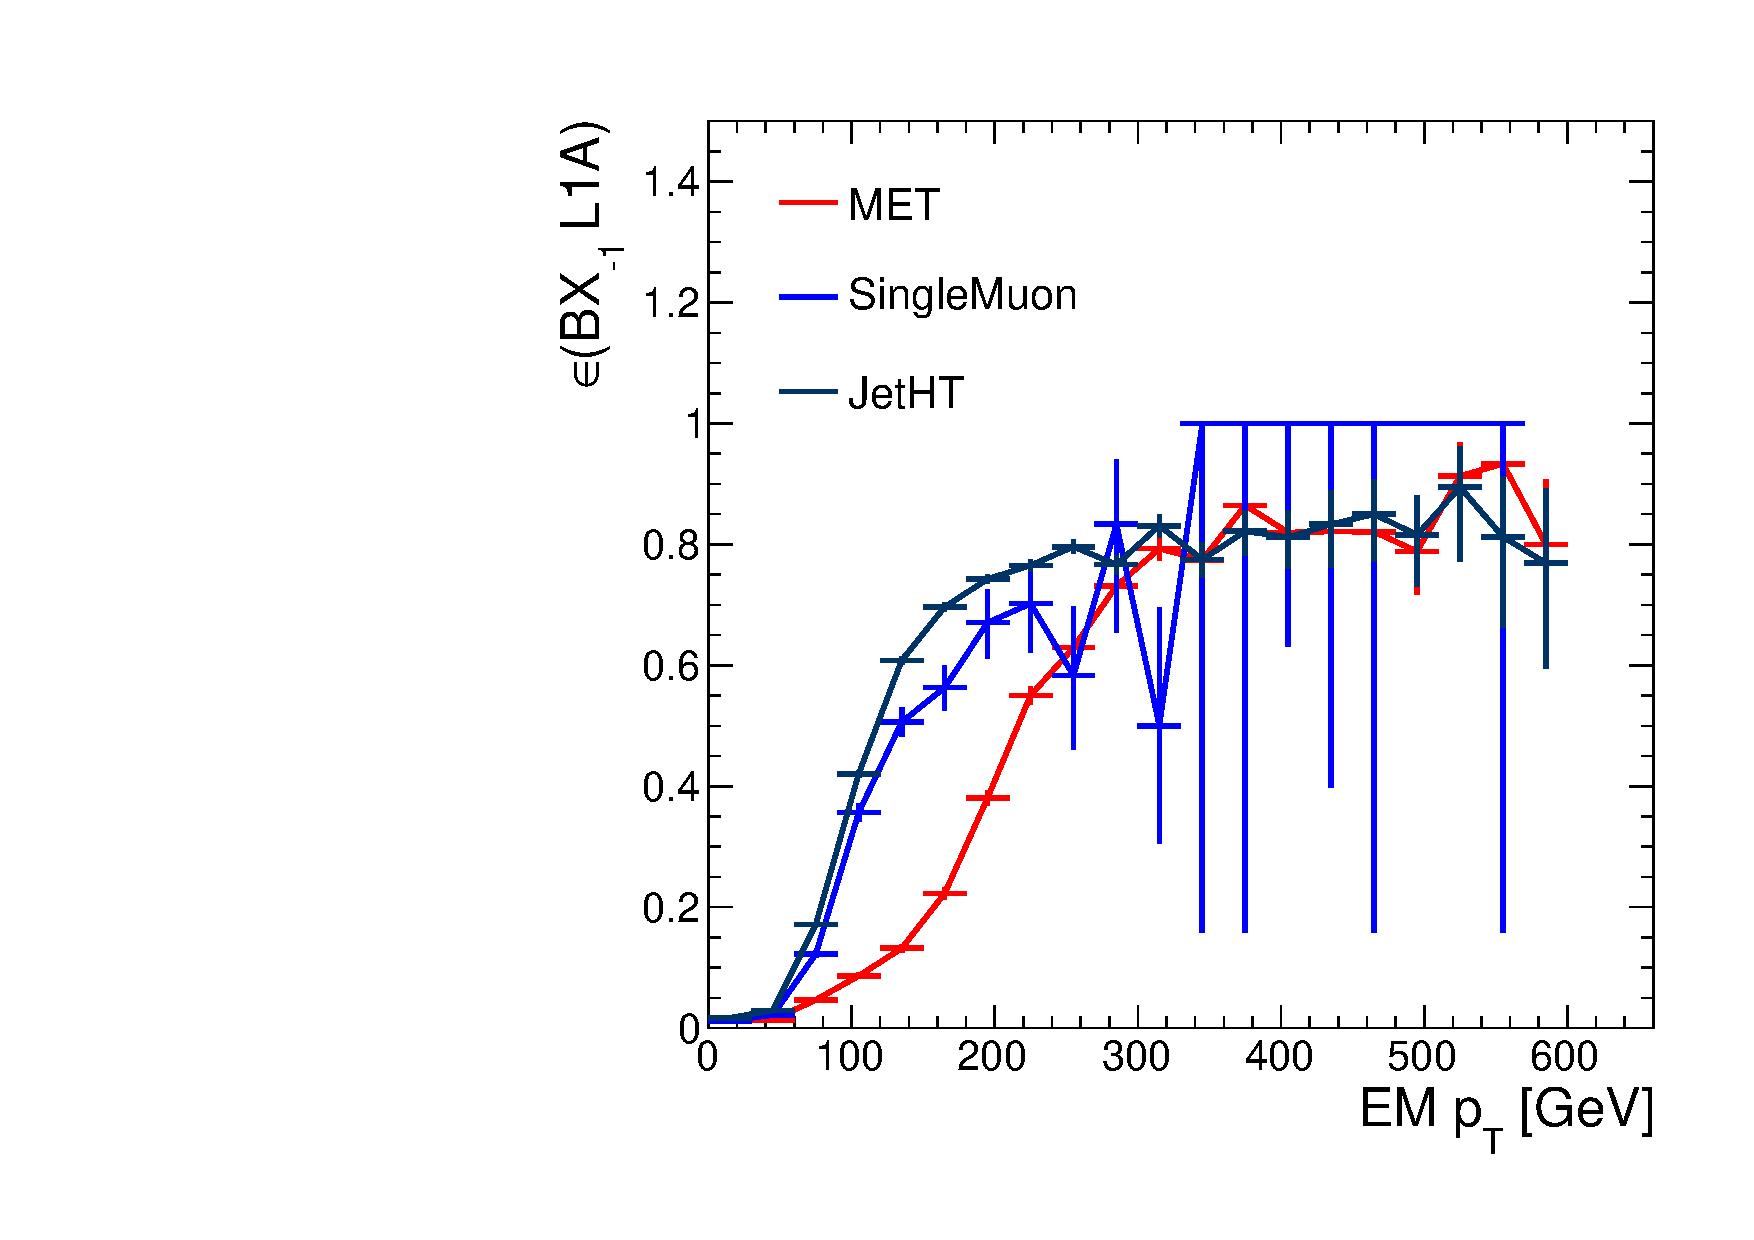
\includegraphics[width=\textwidth]{figures/vbf/triggers/oned_jotEMPt_finor_ratio.pdf}
            \caption{$\pt \times E_\mathrm{ECAL}/E_\mathrm{total}$}
            \label{fig:vbf:hltb}
        \end{subfigure}
        \caption{Probability that a given jet with $2.25<|\eta|<3$ causes a pre-fire in the L1 trigger due to ECAL mistiming.
                 Two parameterizations are used: jet $\pt$ and EM $\pt$.
                 The three curves refer to which set of triggers are used to select $\bx{0}$.}
        \label{fig:vbf:pre_eff1}
    \end{center}
\end{figure}




\subsection{EW and QCD production of electroweak bosons}

\subsection{Sensitivity optimization}

\section{Background estimation}

\section{Results}

\subsection{Constraints on Higgs production and decay parameters}

\subsection{Constraints on scalar production of DM}

